\documentclass[11pt,a4paper]{jarticle}
\usepackage[dvipdfmx]{graphicx}
\usepackage{url}

\renewcommand{\baselinestretch}{1.05} 
\marginparwidth=0cm
\topmargin=-1cm
\headheight=0.3cm
\headsep=0.7cm
\oddsidemargin=0cm
\evensidemargin=0cm
%\textwidth=43zw
\textwidth=15.92cm
%\textheight=43.3\baselineskip
\baselineskip = 0.5744cm
\textheight=43\baselineskip

\itemsep=0.05\baselineskip
\parsep=0pt
\topsep=0.01\baselineskip
\partopsep=0pt
\listparindent=0zw

%% header and footer
\usepackage{fancyhdr}
\pagestyle{fancy}
\lhead{2014年度 春学期授業}
\chead{インタラクティブ・アート実習}
\rhead{担当教員: 松下 光範}
\cfoot{\thepage}
\renewcommand{\headrulewidth}{0pt}
\renewcommand{\footrulewidth}{0pt}

\usepackage{ascmac}
\usepackage{listings,jlisting}
\usepackage{color}
\definecolor{OliveGreen}{cmyk}{0.64,0,0.95,0.40}
\definecolor{colFunc}{rgb}{1,0.07,0.54}
\definecolor{CadetBlue}{cmyk}{0.62,0.57,0.23,0}
\definecolor{Brown}{cmyk}{0,0.81,1,0.60}
\definecolor{colID}{rgb}{0.63,0.44,0}
\definecolor{rulesepcolor}{gray}{0.666}
\lstset{
  language=Java,%プログラミング言語によって変える。
  basicstyle={\ttfamily\small},
  keywordstyle={\color{OliveGreen}},
  %[2][3]はプログラミング言語によってあったり、なかったり
  keywordstyle={[2]\color{colFunc}},
  keywordstyle={[3]\color{CadetBlue}},%
  commentstyle={\color{Brown}},
  %identifierstyle={\color{colID}},
  stringstyle=\color{blue},
  tabsize=2,
  %frame=trBL,
  %numbers=left,
  numberstyle={\ttfamily\small},
  breaklines=true,%折り返し
  %backgroundcolor={\color[gray]{.95}},
  framexleftmargin=0mm,
  frame=single,
  rulesepcolor=\color{rulesepcolor},
  captionpos=b
}


%%%%%%%%%%%%%%%%%%%%%%%%%%%%%%%%%%%%%%%%%%%%%%%%%%%%%%%%%%%%%%%%
\begin{document}

% title
\section*{\LARGE{第2講 プログラミングでLEDを制御する}}
Processing と Arduino を接続し LED を制御する。
スイッチの ON/OFF を取得する。

%%%%%%%%%%%%%%%%%%%%%%%%%%%%%%%%%%%%%%%%%%%%%%%%%%%%%%%%%%%%%%%%


\section{Arduino の準備}
本実習ではスイッチやセンサ、LED などを PC から制御するために Arduino\footnote{\url{http://arduino.cc}} というマイコンを用います。

本来、Arduino と Processing を連携させるためには、シリアル通信を用いますが、そのためのプログラムを書くのは少し面倒です。
実習では楽をするために、Firmata\footnote{\url{http://firmata.org}} を用います。

\subsection*{Todo}
\begin{itemize}
 \item Arduino IDE のインストール
 \item Arduino ドライバのインストール
 \item Arduino に Firmata を書き込む
 \item Processing に Arduino ライブラリをインストール       
 \item 動作確認
\end{itemize}


\section{Processing から Arduino を制御する}
今回は Arduino の Digital Output を用いて LED の制御したり、
Digital Input を用いてスイッチの ON/OFF を取得したりします。

まず、Processing から Arduino を用いるための準備をしましょう。
\begin{lstlisting}
 import processing.serial.*;
 import cc.arduino.*;

 Arduino arduino;

 void setup() {
   // Arduino の初期化
   // シリアルポートの指定など
   // Arduino.list()[0] は環境によって変える
   arduino = new Arduino(this, Arduino.list()[0], 57600);
 }
\end{lstlisting}
Arduino を使うためにはシリアルポートの指定をしなければなりません。
Windows ならデバイスマネージャから確認することができます。
Arduino.list()[0] のところを各自変更してください。

これらの命令は今後も Arduino を用いる際に必ず使うので忘れないように。


\subsection*{LED を点滅させる}
Digital Output を使って LED を点滅させてみましょう。

\subsubsection*{回路を組む}
\begin{figure}[h!]
 \begin{minipage}{0.5\columnwidth}
  LED を接続したピンに電圧をかけると LED が点灯する回路を作りましょう。
  \begin{itemize}
   \item \textbf{使う部品}
	 \begin{itemize}
	  \item Arduino
	  \item 抵抗
	  \item LED
	 \end{itemize}
   \item \textbf{ポイント}
	 \begin{itemize}
	  \item 5V → LED → 抵抗 → GND の順に
	  \item LED には極性があるので向きに注意
	 \end{itemize}
  \end{itemize}
 \end{minipage}
 \begin{minipage}{0.5\columnwidth}
  \centering
  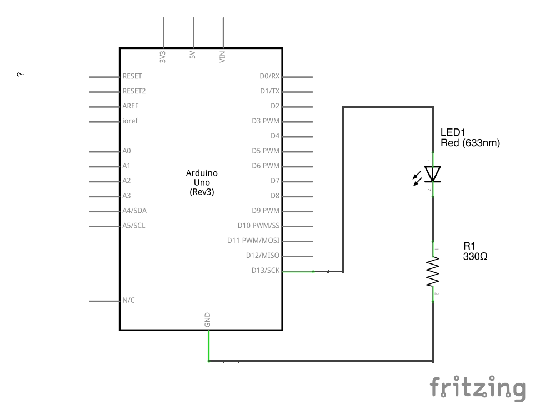
\includegraphics[width=80mm]{img/02_led.eps}
  \caption{回路図}
 \end{minipage}
\end{figure}

\subsubsection*{プログラムを書く}
LED を接続したピンの電圧を制御するプログラムを書きましょう。
\begin{lstlisting}
import processing.serial.*;
import cc.arduino.*;
 
Arduino arduino;
int ledPin = 13; // LED を接続したピンの番号
 
void setup() {
  arduino = new Arduino(this, Arduino.list()[0], 57600);

  // Arduino のピンモードを設定
  // ここでは 13 番ピンを Output 用に設定
  arduino.pinMode(ledPin, Arduino.OUTPUT);
}
 
void draw() {
  // Arduino の 13 番ピンを HIGH (5V) に
  arduino.digitalWrite(ledPin, Arduino.HIGH);
  delay(500); // 500ミリ秒間待つ

  // Arduino の 13 番ピンを LOW (0V) に
  arduino.digitalWrite(ledPin, Arduino.LOW);
  delay(500);
}
\end{lstlisting}
これで LED が点滅するはずです。


\subsection*{スイッチの ON/OFF を読み取る}
Arduino の Digital Input を用いてスイッチの ON/OFF を取得する。

\subsubsection*{回路を組む}
デジタル回路の場合、入力端子がどこにも接続されていないような状態 (オープン) が起こると、電圧が High または Low に定まらず誤動作の原因になります。
そのため、回路を安定させるためにプルアップ抵抗/プルダウン抵抗と呼ばれる抵抗を用います。

\begin{figure}[h!]
 \begin{minipage}{0.5\columnwidth}
  \centering
  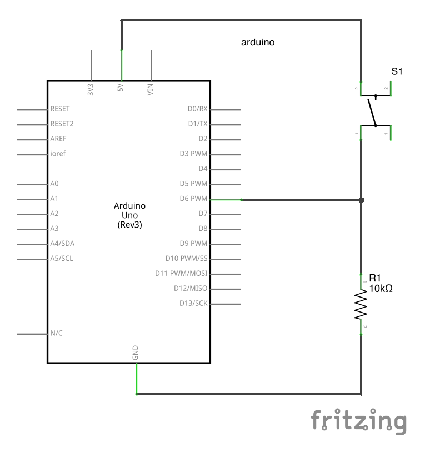
\includegraphics[width=0.7\columnwidth]{img/pulldown.eps}
 \end{minipage}
 \begin{minipage}{0.5\columnwidth}
  \centering
  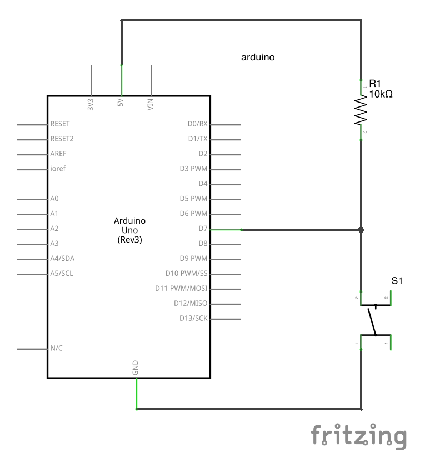
\includegraphics[width=0.7\columnwidth]{img/pullup.eps}
 \end{minipage}
  \caption{プルダウン抵抗 (左) とプルアップ抵抗 (右)}
\end{figure}


\subsubsection*{プログラムを書く}
\begin{lstlisting}
import processing.serial.*;
import cc.arduino.*;

Arduino arduino;
int switchPin = 8; // スイッチを接続したピンの番号
 
void setup() {
  size(400, 300);
  arduino = new Arduino(this, Arduino.list()[0], 57600);
  arduino.pinMode(switchPin, Arduino.INPUT); // ピンモードを Input に
}
 
void draw() {
  // 8 番ピンの電圧を取得し、それが HIGH ならば
  if (arduino.digitalRead(switchPin) == Arduino.HIGH) {
    background(255, 0, 0); // 背景を赤に
  } else {
    background(0, 0, 0);   // そうでなければ (LOW ならば) 背景を黒に
  }
}
\end{lstlisting}


\subsection*{スイッチを押すと LED が点灯するようにする}
スイッチの入力を Processing で取得し、それに基づいて LED を制御しましょう。
上 2 つの合わせ技です。

これで入力と出力の両方が実現できるようになります。
次回以降の実習でも入力や出力のための部品が変わるだけで基本的な考え方は同じです。


\subsubsection*{TRY}
今回やったことを思い出しながら、回路とプログラムを作成してみましょう。

% \subsubsection*{プログラムを書く}
% \begin{lstlisting}
% import processing.serial.*;
% import cc.arduino.*;

% Arduino arduino;
% int ledPin = 13;
% int switchPin = 8;
 
% void setup() {
%   size(400, 300);
%   arduino = new Arduino(this, Arduino.list()[0], 57600);
%   arduino.pinMode(switchPin, Arduino.INPUT);
%   arduino.pinMode(ledPin, Arduino.OUTPUT);
% }
 
% void draw() {
%   if (arduino.digitalRead(switchPin) == Arduino.HIGH) {
%     background(255, 0, 0);
%     arduino.digitalWrite(ledPin, Arduino.HIGH);
%   } else {
%     background(0, 0, 0);
%     arduino.digitalWrite(ledPin, Arduino.LOW);
%   }
% }
% \end{lstlisting}

\end{document}
